\documentclass[aspectratio=169,11pt]{beamer}
% Shared style for the Introduction to Information Geometry lecture slides.
% Compile the lecture .tex files from this directory.
\providecommand{\courseweek}{1}
\usepackage[T1]{fontenc}
\usepackage[utf8]{inputenc}
\usepackage[sc]{mathpazo}
\renewcommand{\sfdefault}{lmss}
\renewcommand{\ttdefault}{lmtt}
\usepackage{amsmath,amssymb,mathtools}
\usepackage{tikz}
\usetikzlibrary{arrows.meta,calc,positioning}
\usepackage{pgfplots}
\pgfplotsset{compat=1.18}
\usepackage{booktabs}

\definecolor{courseink}{HTML}{173749}
\definecolor{coursemuted}{HTML}{526674}
\definecolor{courseteal}{HTML}{0E7287}
\definecolor{coursecopper}{HTML}{B66B43}
\definecolor{courseline}{HTML}{D4E0E3}
\definecolor{coursepale}{HTML}{EFF5F5}

\setbeamercolor{normal text}{fg=courseink,bg=white}
\setbeamercolor{structure}{fg=courseteal}
\setbeamercolor{frametitle}{fg=courseink,bg=white}
\setbeamercolor{title}{fg=courseink}
\setbeamercolor{subtitle}{fg=coursemuted}
\setbeamercolor{block title}{fg=courseink,bg=white}
\setbeamercolor{block body}{fg=courseink,bg=white}
\setbeamercolor{alerted text}{fg=coursecopper}
\setbeamerfont{title}{family=\rmfamily,series=\bfseries,size=\fontsize{32}{37}}
\setbeamerfont{frametitle}{family=\rmfamily,series=\bfseries,size=\fontsize{26}{31}}
\setbeamerfont{normal text}{size=\fontsize{18}{22}}
\setbeamerfont{subtitle}{size=\fontsize{17}{21}}
\setbeamersize{text margin left=0.78cm,text margin right=0.78cm}
\setbeamertemplate{navigation symbols}{}
\setbeamertemplate{itemize items}[circle]
\setbeamertemplate{enumerate items}[default]
\setbeamertemplate{blocks}[default]
\setlength{\parskip}{0.22em}
\setbeamertemplate{footline}{%
  \leavevmode\hbox to \paperwidth{\hspace{.78cm}%
  {\color{coursemuted}\fontsize{8.5}{10}\selectfont Introduction to Information Geometry \hspace{.32cm} / \hspace{.32cm} Week \courseweek}%
  \hfill{\color{coursemuted}\fontsize{8.5}{10}\selectfont \insertframenumber\hspace{.17cm}/\hspace{.17cm}\inserttotalframenumber}\hspace{.78cm}}%
  \vskip.17cm
}
\setbeamertemplate{frametitle}{%
  \vspace{.13cm}
  \insertframetitle\par
  \vspace{.08cm}
}
\setbeamertemplate{title page}{%
  \vspace*{1.00cm}
  {\color{courseteal}\fontsize{10}{13}\selectfont\bfseries
  INTRODUCTION TO INFORMATION GEOMETRY\par}
  \vspace{.40cm}
  {\usebeamerfont{title}\usebeamercolor[fg]{title}\inserttitle\par}
  \vspace{.22cm}
  {\usebeamerfont{subtitle}\usebeamercolor[fg]{subtitle}\insertsubtitle\par}
  \vfill
  {\color{coursemuted}\fontsize{13}{16}\selectfont Christopher Lee\par}
  \vspace{.34cm}
}

\pgfplotsset{
  courseplot/.style={
    width=11.05cm,
    height=5.15cm,
    axis line style={coursemuted!75},
    tick style={coursemuted!65},
    ticklabel style={font=\scriptsize,color=coursemuted},
    label style={font=\normalsize,color=courseink},
    grid=major,
    major grid style={courseline!70,line width=.4pt},
    line width=1.45pt,
    legend style={font=\small,draw=none,fill=none,at={(.98,.03)},anchor=south east},
    clip=true
  }
}

\newcommand{\highlightmath}[1]{{\color{courseteal}#1}}
\newcommand{\thinrule}{\par\vspace{.25cm}{\color{courseline}\rule{\linewidth}{.8pt}}\par}

% A one-dimensional state space.  x=0 and x=1 are placed at 0 and 9 units.
\newcommand{\stateinterval}[1]{%
 \begin{tikzpicture}[x=1cm,y=1cm]
   \draw[courseink,line width=1.25pt] (0,0)--(9,0);
   \foreach \pos/\lab in {0/0,9/1} {
     \fill[courseink] (\pos,0) circle(2.7pt);
     \node[below=9pt,text=coursemuted] at (\pos,0) {\(\lab\)};
   }
   #1
 \end{tikzpicture}%
}

% Paired pages are separate frames in the PDF, with matching titles.
% Supply the whole frame body for each version; the instructor may edit them
% independently without changing overlay logic.
\newcommand{\coursepair}[3]{%
  \begin{frame}{#1}#2\end{frame}%
  \begin{frame}{#1}#3\end{frame}%
}

% Equilateral representation of the categorical simplex, in barycentric
% coordinates with vertices A=(0,0), B=(1,0), C=(1/2,sqrt(3)/2).
\newcommand{\coursesimplex}[1]{%
 \begin{tikzpicture}[scale=4.9]
  \fill[coursepale] (0,0)--(1,0)--(.5,.8660254)--cycle;
  \draw[courseink,line width=.65pt] (0,0)--(1,0)--(.5,.8660254)--cycle;
  \node[below left,font=\small] at (0,0) {A};
  \node[below right,font=\small] at (1,0) {B};
  \node[above,font=\small] at (.5,.8660254) {C};
  #1
 \end{tikzpicture}%
}

\title{Population Proportions\\and Replicator Dynamics}
\subtitle{Week 1 \(\cdot\) Lecture 1}
\date{}

\begin{document}

% 1
\begin{frame}[plain]
\titlepage
\end{frame}

% 2
\begin{frame}{Counts and proportions}
Two observations of a population:
\vspace{.32cm}

\begin{center}
\begin{tabular}{@{}lrrr@{}}
& Type A & Type B & Total\\
\midrule
First census & 48 & 72 & 120\\
Second census & 90 & 180 & 270
\end{tabular}
\end{center}
\vspace{.35cm}
\begin{center}

\begin{tikzpicture}[x=1cm,y=1cm]
  \node[anchor=east,text=coursemuted] at (0,1.1) {First};
  \node[anchor=east,text=coursemuted] at (0,0) {Second};
  \fill[courseteal] (0,0.82) rectangle (3.6,1.35);
  \fill[coursecopper!70] (3.6,.82) rectangle (9,1.35);
  \fill[courseteal] (0,-.28) rectangle (3,-.28+.53);
  \fill[coursecopper!70] (3,-.28) rectangle (9,-.28+.53);
  \node[white,font=\bfseries] at (1.8,1.085) {\(?\)};
  \node[white,font=\bfseries] at (6.3,1.085) {\(?\)};
  \node[white,font=\bfseries] at (1.5,-.015) {\(?\)};
  \node[white,font=\bfseries] at (6,-.015) {\(?\)};
\end{tikzpicture}
\end{center}
Which type gained in number? Which gained in share?
\end{frame}

% Reveal: counts and proportions
\begin{frame}{Counts and proportions}
Two observations of a population:
\vspace{.32cm}

\begin{center}
\begin{tabular}{@{}lrrr@{}}
& Type A & Type B & Total\\
\midrule
First census & 48 & 72 & 120\\
Second census & 90 & 180 & 270
\end{tabular}
\end{center}
\vspace{.35cm}
\begin{center}

\begin{tikzpicture}[x=1cm,y=1cm]
  \node[anchor=east,text=coursemuted] at (0,1.1) {First};
  \node[anchor=east,text=coursemuted] at (0,0) {Second};
  \fill[courseteal] (0,0.82) rectangle (3.6,1.35);
  \fill[coursecopper!70] (3.6,.82) rectangle (9,1.35);
  \fill[courseteal] (0,-.28) rectangle (3,-.28+.53);
  \fill[coursecopper!70] (3,-.28) rectangle (9,-.28+.53);
  \node[white,font=\bfseries] at (1.8,1.085) {40\% A};
  \node[white,font=\bfseries] at (6.3,1.085) {60\% B};
  \node[white,font=\bfseries] at (1.5,-.015) {33.3\% A};
  \node[white,font=\bfseries] at (6,-.015) {66.7\% B};
\end{tikzpicture}
\end{center}
Both types grew in number. Type B gained in share.
\end{frame}

% 3
\begin{frame}{One variable describes the composition}
\vspace{.06cm}
\[
\highlightmath{x(t)=\frac{N_A(t)}{N_A(t)+N_B(t)}},
\qquad 1-x(t)=\frac{N_B(t)}{N_A(t)+N_B(t)}.
\]
\vspace{.20cm}
\begin{center}
\stateinterval{
  \fill[courseteal] (3.6,0) circle (4pt);
  \draw[courseteal,line width=.9pt] (3.6,0)--(3.6,.62);
  \node[above,text=courseteal] at (3.6,.62) {\(x=0.4\)};
  \node[above,text=coursemuted] at (0,.10) {Only B};
  \node[above,text=coursemuted] at (9,.10) {Only A};
}
\end{center}
\vspace{.18cm}
\begin{center}
The state space of the proportion is \(\highlightmath{[0,1]}\).
\end{center}
\end{frame}

% 4
\begin{frame}{Many populations share one composition}
\begin{center}
\vspace{.15cm}
\[
(N_A,N_B)=(20,30),
\qquad (200,300),
\qquad (2000,3000)
\]
\vspace{.12cm}
\[
\highlightmath{x=\frac{N_A}{N_A+N_B}=\frac25}
\]
\vspace{.12cm}
\end{center}
Multiplying both counts by the same positive number leaves \(x\) unchanged.

\vspace{.20cm}
The proportion describes relative abundance while the total
\(N=N_A+N_B\) records population size.
\end{frame}

% 5
\begin{frame}{Growth equations for the two types}
Let \(f_A\) and \(f_B\) be the per-capita growth rates.
\vspace{.45cm}
\[
\boxed{N_A'=f_A N_A \qquad N_B'=f_B N_B}
\]
\vspace{.5cm}
\begin{itemize}
  \setlength{\itemsep}{.5cm}
  \item \(f_A>0\) means type A increases in number.
  \item \(f_A<0\) means type A decreases in number.
  \item The units of each \(f_i\) are inverse time.
\end{itemize}
\end{frame}

% 6
\begin{frame}{Differentiating the proportion}
Write \(N=N_A+N_B\), so \(x=N_A/N\).
\vspace{.55cm}
\[
x'=\frac{N_A'N-N_A N'}{N^2}.
\]
\vspace{.46cm}
\[
N'=\,?
\qquad\qquad
x'=\;?
\]
\end{frame}

% Reveal: differentiating the proportion
\begin{frame}{Differentiating the proportion}
Write \(N=N_A+N_B\), so \(x=N_A/N\).
\vspace{.55cm}
\[
x'=\frac{N_A'N-N_A N'}{N^2}.
\]
\vspace{.36cm}
\[
N'=f_A N_A+f_B N_B
\]
\vspace{.16cm}
\[
x'=\frac{N_A N_B}{N^2}(f_A-f_B).
\]
\end{frame}

% 7
\begin{frame}{The two-strategy replicator equation}
\vspace{.6cm}
\begin{center}
{\fontsize{30}{36}\selectfont
\(\displaystyle \highlightmath{x'=x(1-x)(f_A-f_B)}\)}
\end{center}
\vspace{.55cm}
\begin{columns}[T,onlytextwidth]
\column{.30\textwidth}
\centering \(x\)\\[.18cm]\small Current share of A
\column{.30\textwidth}
\centering \(1-x\)\\[.18cm]\small Current share of B
\column{.37\textwidth}
\centering \(f_A-f_B\)\\[.18cm]\small Relative fitness advantage
\end{columns}
\vspace{.65cm}
\centering The sign of \(x'\) describes which type is gaining proportion.
\end{frame}

% 8
\begin{frame}{Relative advantage controls direction}
For an interior state, \(0<x<1\), the factor \(x(1-x)\) is positive.
\vspace{.45cm}
\[
\begin{array}{rcl}
f_A>f_B &\Longrightarrow& x'>0 \\[.5cm]
f_A<f_B &\Longrightarrow& x'<0 \\[.5cm]
f_A=f_B &\Longrightarrow& x'=0
\end{array}
\]
\vspace{.6cm}
The two counts may both increase or both decrease. Their \emph{difference
in per-capita rates} determines the change in composition.
\end{frame}

% 9
\begin{frame}{A declining population}
At a particular time, suppose
\vspace{.27cm}
\[
x=0.4,\qquad f_A=-0.1,\qquad f_B=-0.4
\quad(\text{per day}).
\]
\vspace{.25cm}
Find the instantaneous rate of change of the proportion:
\[
x'=x(1-x)(f_A-f_B)=\underline{\hspace{2cm}}.
\]
\vspace{.3cm}
Then calculate the total population's per-capita growth rate
\[
\frac{N'}{N}=xf_A+(1-x)f_B=\underline{\hspace{2cm}}.
\]
\end{frame}

% Reveal: declining population
\begin{frame}{A declining population}
At a particular time, suppose
\vspace{.27cm}
\[
x=0.4,\qquad f_A=-0.1,\qquad f_B=-0.4
\quad(\text{per day}).
\]
\vspace{.25cm}
Find the instantaneous rate of change of the proportion:
\[
x'=x(1-x)(f_A-f_B)=\highlightmath{0.072}\ \text{day}^{-1}.
\]
\vspace{.3cm}
Then calculate the total population's per-capita growth rate
\[
\frac{N'}{N}=xf_A+(1-x)f_B=\highlightmath{-0.28}\ \text{day}^{-1}.
\]
Type A gains share while the total population declines.
\end{frame}

% 10
\begin{frame}{Constant fitness advantage}
Suppose the difference \(f_A-f_B=k\) is constant.
\vspace{.42cm}
\[
\highlightmath{x'=kx(1-x)}.
\]
\vspace{.38cm}
\begin{itemize}
 \setlength{\itemsep}{.48cm}
 \item \(k>0\): A increases its share from every interior state.
 \item \(k<0\): B increases its share from every interior state.
 \item \(k=0\): every composition is stationary.
\end{itemize}
\end{frame}

% 11
\begin{frame}{Phase lines for constant advantage}
\vspace{.20cm}
\begin{center}
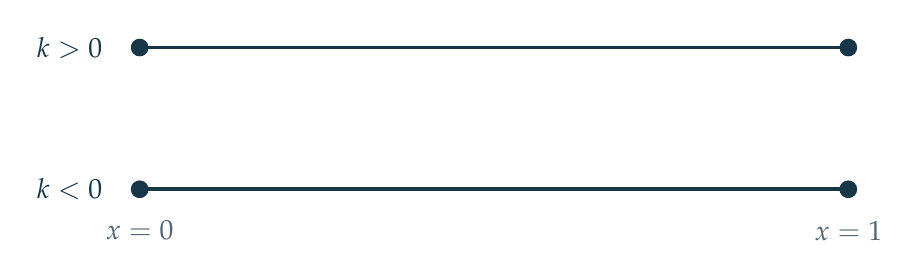
\begin{tikzpicture}[x=1cm,y=1cm]
 \node[anchor=east,text=courseink] at (-.35,1.2) {\(k>0\)};
 \draw[courseink,line width=1.35pt] (0,1.2)--(9,1.2);
 \fill[courseink] (0,1.2) circle(3.2pt);
 \fill[courseink] (9,1.2) circle(3.2pt);
 \node[anchor=east,text=courseink] at (-.35,-.6) {\(k<0\)};
 \draw[courseink,line width=1.35pt] (0,-.6)--(9,-.6);
 \fill[courseink] (0,-.6) circle(3.2pt);
 \fill[courseink] (9,-.6) circle(3.2pt);
 \node[below,text=coursemuted] at (0,-.88) {\(x=0\)};
 \node[below,text=coursemuted] at (9,-.88) {\(x=1\)};
\end{tikzpicture}
\end{center}
\vspace{.30cm}
Draw the direction arrows. Which endpoint attracts for each sign of \(k\)?
\end{frame}

% Reveal: constant-advantage phase lines
\begin{frame}{Phase lines for constant advantage}
\vspace{.20cm}
\begin{center}
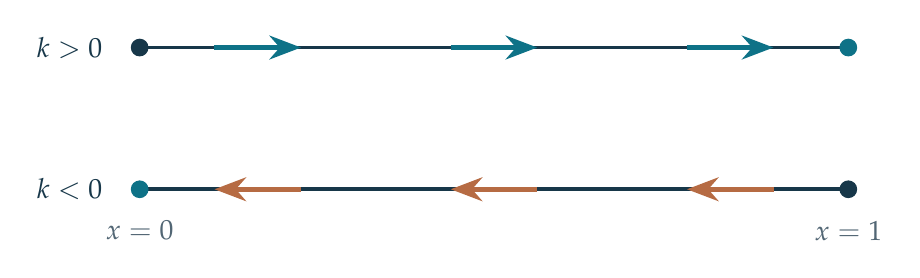
\begin{tikzpicture}[x=1cm,y=1cm]
 \node[anchor=east,text=courseink] at (-.35,1.2) {\(k>0\)};
 \draw[courseink,line width=1.35pt] (0,1.2)--(9,1.2);
 \fill[courseink] (0,1.2) circle(3.2pt);
 \fill[courseteal] (9,1.2) circle(3.2pt);
 \foreach \x in {1.5,4.5,7.5}
   \draw[-{Stealth[length=4mm]},courseteal,line width=2pt] (\x-.55,1.2)--(\x+.55,1.2);
 \node[anchor=east,text=courseink] at (-.35,-.6) {\(k<0\)};
 \draw[courseink,line width=1.35pt] (0,-.6)--(9,-.6);
 \fill[courseteal] (0,-.6) circle(3.2pt);
 \fill[courseink] (9,-.6) circle(3.2pt);
 \foreach \x in {1.5,4.5,7.5}
   \draw[-{Stealth[length=4mm]},coursecopper,line width=2pt] (\x+.55,-.6)--(\x-.55,-.6);
 \node[below,text=coursemuted] at (0,-.88) {\(x=0\)};
 \node[below,text=coursemuted] at (9,-.88) {\(x=1\)};
\end{tikzpicture}
\end{center}
\vspace{.30cm}
Filled teal endpoints attract trajectories from the interior.
\end{frame}

% 12
\begin{frame}{The logistic velocity field}
\vspace{-.25cm}
\begin{center}
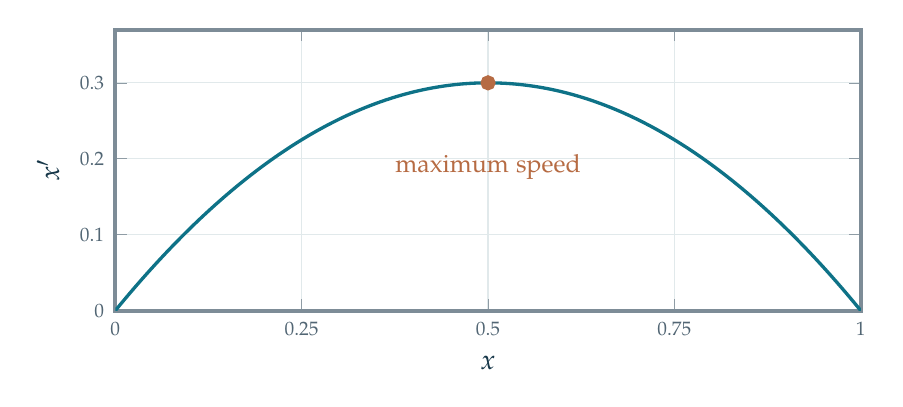
\begin{tikzpicture}
\begin{axis}[courseplot,xmin=0,xmax=1,ymin=0,ymax=.37,
 xlabel={$x$},ylabel={$x'$},xtick={0,.25,.5,.75,1},
 ytick={0,.1,.2,.3}]
\addplot[courseteal,very thick,domain=0:1,samples=150] {1.2*x*(1-x)};
\addplot[only marks,mark=*,mark size=2pt,coursecopper] coordinates {(.5,.3)};
\node[anchor=north,text=coursecopper,font=\small] at (axis cs:.5,.22) {maximum speed};
\end{axis}
\end{tikzpicture}
\end{center}
\vspace{-.17cm}
For \(x'=1.2x(1-x)\), motion slows near either endpoint.
\end{frame}

% 13
\begin{frame}{Solution curves in time}
\vspace{-.3cm}
\begin{center}
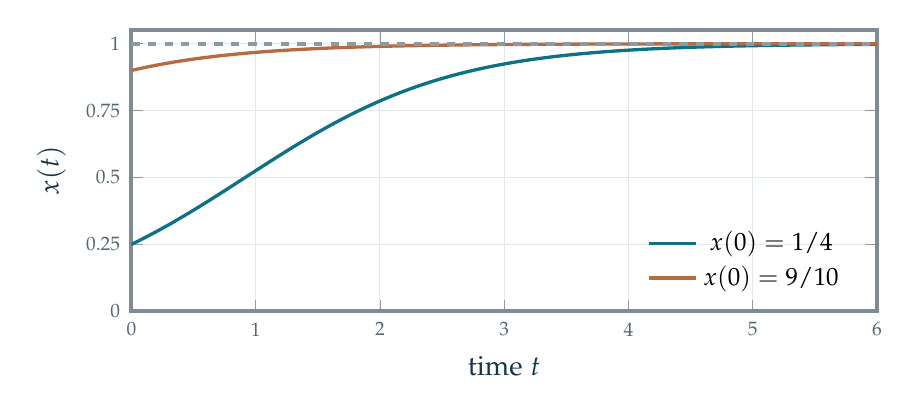
\begin{tikzpicture}
\begin{axis}[courseplot,xmin=0,xmax=6,ymin=0,ymax=1.05,
 xlabel={time \(t\)},ylabel={$x(t)$},xtick={0,1,2,3,4,5,6},
 ytick={0,.25,.5,.75,1},legend pos=south east]
\addplot[courseteal,very thick,domain=0:6,samples=160] {1/(1+3*exp(-1.2*x))};
\addlegendentry{\(x(0)=1/4\)}
\addplot[coursecopper,very thick,domain=0:6,samples=160] {1/(1+(1/9)*exp(-1.2*x))};
\addlegendentry{\(x(0)=9/10\)}
\addplot[courseink!50,dashed,domain=0:6] {1};
\end{axis}
\end{tikzpicture}
\end{center}
\vspace{-.14cm}
The phase line gives direction. The initial condition determines a particular curve.
\end{frame}

% 14
\begin{frame}{Solving the logistic equation}
For an interior solution of \(x'=kx(1-x)\),
\vspace{.36cm}
\[
\frac{dx}{x(1-x)}=k\,dt.
\]
\vspace{.25cm}
Use partial fractions:
\[
\frac1{x(1-x)}=\frac1x+\frac1{1-x}.
\]
\vspace{.25cm}
\[
\int\frac{dx}{x(1-x)}=\underline{\hspace{4cm}}.
\]
\end{frame}

% Reveal: separation of variables
\begin{frame}{Solving the logistic equation}
For an interior solution of \(x'=kx(1-x)\),
\vspace{.36cm}
\[
\frac{dx}{x(1-x)}=k\,dt.
\]
\vspace{.25cm}
Use partial fractions:
\[
\frac1{x(1-x)}=\frac1x+\frac1{1-x}.
\]
\vspace{.25cm}
\[
\int\frac{dx}{x(1-x)}=\highlightmath{\ln\frac{x}{1-x}=kt+C}.
\]
\end{frame}

% 15
\begin{frame}{The explicit logistic solution}
\vspace{.65cm}
\begin{center}
{\fontsize{27}{35}\selectfont
\(\displaystyle
\highlightmath{x(t)=\frac{1}{1+\frac{1-x_0}{x_0}\,e^{-kt}}}
\)}
\end{center}
\vspace{.65cm}
For \(0<x_0<1\), \(k>0\) gives \(x(t)\to1\) as \(t\to\infty\).
\vspace{.5cm}
The endpoint states \(x_0=0\) and \(x_0=1\) are constant solutions.
\end{frame}

% 16
\begin{frame}{Time to an equal mixture}
Suppose
\[
x'=1.2x(1-x), \qquad x(0)=\frac14.
\]
\vspace{.35cm}
At what time does the proportion first reach \(x=\frac12\)?
\vspace{.40cm}
\[
\frac12=\frac{1}{1+3e^{-1.2t}}
\]
\vspace{.3cm}
\[
t=\underline{\hspace{3.2cm}}.
\]
\end{frame}

% Reveal: time to equal mixture
\begin{frame}{Time to an equal mixture}
Suppose
\[
x'=1.2x(1-x), \qquad x(0)=\frac14.
\]
\vspace{.35cm}
At what time does the proportion first reach \(x=\frac12\)?
\vspace{.40cm}
\[
\frac12=\frac{1}{1+3e^{-1.2t}}
\]
\vspace{.3cm}
\[
\highlightmath{t=\frac{\ln 3}{1.2}\approx0.916}\text{ time units}.
\]
\end{frame}

% 18
\begin{frame}{Composition and total growth}
Two fitness pairs can give the same proportion equation:
\vspace{.23cm}
\[
(f_A,f_B)=(1,0)\qquad\text{and}\qquad(2,1).
\]
\vspace{.28cm}
Both have \(f_A-f_B=1\), hence both produce
\[
\highlightmath{x'=x(1-x)}.
\]
\vspace{.30cm}
Their totals grow at different rates, because
\[
\frac{N'}N=xf_A+(1-x)f_B.
\]
\vspace{.30cm}
The composition equation retains relative growth information.
\end{frame}

\end{document}
